\documentclass[10pt]{article}
\usepackage{fullpage}
\usepackage{amsmath}
\usepackage[amsthm, thmmarks]{ntheorem}
\usepackage{amssymb}
\usepackage{graphicx}
\usepackage{enumerate}
\usepackage{verse}
\usepackage{tikz}
\usepackage{verbatim}
\usepackage{hyperref}

\newtheorem{lemma}{Lemma}
\newtheorem{theorem}[lemma]{Theorem}
\newtheorem{definition}[lemma]{Definition}
\newtheorem{proposition}[lemma]{Proposition}
\newtheorem{corollary}[lemma]{Corollary}
\newtheorem{claim}[lemma]{Claim}
\newtheorem{example}[lemma]{Example}

\newcommand{\dee}{\mathrm{d}}
\newcommand{\Dee}{\mathrm{D}}
\newcommand{\In}{\mathrm{in}}
\newcommand{\Out}{\mathrm{out}}
\newcommand{\pdf}{\mathrm{pdf}}
\newcommand{\Cov}{\mathrm{Cov}}
\newcommand{\Var}{\mathrm{Var}}

\newcommand{\ve}[1]{\mathbf{#1}}
\newcommand{\mrm}[1]{\mathrm{#1}}
\newcommand{\etal}{{et~al.}}
\newcommand{\sphere}{\mathbb{S}^2}
\newcommand{\modeint}{\mathcal{M}}
\newcommand{\azimint}{\mathcal{N}}
\newcommand{\ra}{\rightarrow}
\newcommand{\mcal}[1]{\mathcal{#1}}
\newcommand{\X}{\mathcal{X}}
\newcommand{\Y}{\mathcal{Y}}
\newcommand{\Z}{\mathcal{Z}}
\newcommand{\x}{\mathbf{x}}
\newcommand{\y}{\mathbf{y}}
\newcommand{\z}{\mathbf{z}}
\newcommand{\tr}{\mathrm{tr}}
\newcommand{\sgn}{\mathrm{sgn}}
\newcommand{\diag}{\mathrm{diag}}
\newcommand{\Real}{\mathbb{R}}
\newcommand{\sseq}{\subseteq}
\newcommand{\ov}[1]{\overline{#1}}

\title{Polarization}
\author{Pramook Khungurn}

\begin{document}
	\maketitle

	This document is written as I read a small booklet called ``Field Guide to Polarization'' by Edward Collett.  This is done so that I take the time to remember the symbols and terms.

	\section{Foundations of Polarized Light}

	\begin{itemize}
		\item In 1670, \emph{Bartholinus} discovered that wne a single ray of natural incident light propagated through a rhombohedral calcite crystal, to rays emerged.  This demonstrated that a single ray of light actually consists of two rays.

		\item Because the two rays refract at different angles, calcite crystal is said to be double refractive or \textbf{birefringent}.  That is, the two rays experience different refractive indices.

		\item \emph{Huygens} put another crystal to receive the two rays.
		\begin{itemize}
		 	\item He rotated the second crytal and found that he could get the intensity of one ray to maximize and the other to vanish.
		 	\item Rotating $90^\circ$ from that angle, the second ray's intensity is maximized while the first ray's intensity vanishes.  
		 	\item At $45^\circ$, the intensities of the two rays are equal.
		\end{itemize} 

		\item Because the opposite behavior with respect to rotation, the two rays are said to be \textbf{polarized}.  The two polarization states are called the \textbf{s-} and \textbf{p-polarization} states.  The p and s notation from the German words for parallel (paralelle) and perpendicular (senkrecht).

		\item In 1808, \emph{Malus} made the following discoveries and proposals:
		\begin{itemize}
			\item Natural incident light became polarized when it was reflected by a glass surface.
			\item The light reflected close to the incident angle of $57^\circ$ is extinguished when viewed through a calcite crystal.
			\item Malus proposed that the s- and p-polarization are \emph{perpendicular} to each other.
			\item The intensity of the reflected light varied from a maximum to a mininum as the crystal was rotated.
			\item Malus poposed that the amplitude of the reflected beam must be
			$$ A = A_0 \cos\theta.$$
			\item However, intensity is given by the square of the amplitude.  Hence, the intensity is given by:
			\begin{align*}
				I(\theta) = I_0 \cos^2\theta
			\end{align*}
			where $I_0 = A_0^2$.  This is called \textbf{Malus's law}.
		\end{itemize}

		\item In 1812, \emph{Brester} made the following discoveries and proposals
		\begin{itemize}			
			\item For different glasses, after passing the reflected ray through an analyzing calcite crystal, the p-polarized ray vanishes completely when the incident light's angle is at a particular angle $i$.
			\item By rotating the analyzing calcite crystal through $90^\circ$, the s-polarized ray also vanishes.
			\item The refracted ra angle $r$ is simply related to the angle $i$ by:
			\begin{align*}
				i + r = 90^\circ.
			\end{align*}
			\item By Snell's law:
			\begin{align*}
				n_1 \sin i &= n_2 \sin r \\
				n_1 \sin i &= n_2 \sin (90^\circ - i) \\
				n_1 \sin i &= n_2 \cos i \\
				\tan i &= \frac{n_2}{n_1} = n.
			\end{align*}
			This equation is known as \textbf{Brewster's law}, and the angle $i$ is called the \textbf{Brewster's angle}.
			\item Brewster's law allows the index of refraction of a glass to be determined by reflection rather than refraction.
		\end{itemize}
	\end{itemize}

	\section{The Wave Theory of Light}
	\begin{itemize}
		\item In 1820, \emph{Fresnel} came up with \textbf{Fresnel's wave theory}.
		\begin{itemize}
			\item  The opticla field consisted of only two orthogonal components in the plane transverse to the direction of propagation.
			\item The field components are described by the following two \textbf{wave equations}:
			\begin{align*}
				\nabla^2 E_x(\ve{r}, t) &= \frac{1}{v^2} \frac{\partial^2 E_x(\ve{r},t)}{\partial t^2} \\
				\nabla^2 E_y(\ve{r}, t) &= \frac{1}{v^2} \frac{\partial^2 E_y(\ve{r},t)}{\partial t^2}
			\end{align*}
			where
			\begin{itemize}
			 	\item $E_x(\ve{r},t)$ and $E_y(\ve{r},t)$ are the optical-field components, 
			 	\item $\ve{r}$ is a position in space,
			 	\item $t$ is the time, and
			 	\item $v$ is the velocity of the weave.
			\end{itemize}

			\item The solutions of the wave equations are:
			\begin{align*}
				E_x(\ve{r},t) &= E_{0x}\cos(\omega t - \ve{k} \cdot \ve{r} + \delta_x) \\
				E_y(\ve{r},t) &= E_{0y}\cos(\omega t - \ve{k} \cdot \ve{r} + \delta_y)
			\end{align*}
			where
			\begin{itemize}
			 	\item $\ve{k}$ is the (vector) wave number and describes the direction of propagation, 
			 	\item $\omega = 2\pi f$ is the angular frequency, and
			 	\item $\delta_x$ and $\delta_y$ are arbitrary phase offsets.
			\end{itemize} 
			The vector $\ve{k}$ is perpendicular to the plane containing $E_x$ and $E_y$.

			\item In practice, we often assume that the wave propagates along the $z$-direction, i.e., $\ve{k} = (0,0,k)$.  Here, $k = 2\pi/\lambda$ is the wave number magnitude.  So, the solutions become:
			\begin{align*}
				E_x(z,t) &= E_{0x} \cos(\omega t - kz + \delta_x) \\
				E_y(z,t) &= E_{0y} \cos(\omega t - kz + \delta_y).
			\end{align*} 
			The term $\omega t - kz$ is called the \textbf{propagator}.

			\item We may also express the components with the following complex functions:
			\begin{align*}
				\mathcal{E}_x(z,t) &= E_{0x} \exp(i (\omega t - kz + \delta_x)), \\
				\mathcal{E}_y(z,t) &= E_{0y} \exp(i (\omega t - kz + \delta_y)).
			\end{align*}
			Using the functions, we have that
			\begin{align*}
				E_x(z,t) &= \Re \{ \mathcal{E}_x(z,t) \}, \\
				E_y(z,t) &= \Re \{ \mathcal{E}_y(z,t) \}.
			\end{align*}

			\item The $E_y$ component is called the p-polarization component, and $E_x$ is called the s-polarization component.
		\end{itemize}

		\item The two components of the light field satisfies the following equation of an ellipse, called the \textbf{polarization ellipse}:
		\begin{align*}
			\frac{E_x(z,t)^2}{E_{0x}^2} + \frac{E_y(z,t)^2}{E_{0y}^2} - \frac{2 E_x(z,t) E_y(z,t)}{E_{0x} E_{0y}}\cos\delta = \sin^2 \delta
		\end{align*}
		where $\delta = \delta_y - \delta_x$.  The polarization ellipse remains constant as the polarized beam propagate.

		\item There are several combinations of amplitude and phase that are especially important, and they are called \textbf{degenerate polarization states}.
		\begin{itemize}
			\item \textbf{Linearly horizontal polarized light (LHP)}. $E_{0y} = 0$.
			\begin{center}
				\begin{tikzpicture}
					\draw [<->] (-0.5,0) -- (0.5,0);
					\draw [<->,white] (0,-0.5) -- (0,0.5);
				\end{tikzpicture}
			\end{center}
			\item \textbf{Linearly vertical polarized light (LVP)}. $E_{0x} = 0$.
			\begin{center}
				\begin{tikzpicture}
					\draw [<->] (0,-0.5) -- (0,0.5);
				\end{tikzpicture}
			\end{center}
			\item \textbf{Linear $+45^\circ$ polarized light (L+45P)}. $E_{0x} = E_{0y} = E_0$ and $\delta = 0$.
			\begin{center}
				\begin{tikzpicture}
					\draw [<->] (-0.5,-0.5) -- (0.5,0.5);
				\end{tikzpicture}
			\end{center}
			\item \textbf{Linear $-45^\circ$ polarized light (L-45P)}.
			$E_{0x} = E_{0y} = E_0$ and $\delta = \pi$.
			\begin{center}
				\begin{tikzpicture}
					\draw [<->] (0.5,-0.5) -- (-0.5,0.5);
				\end{tikzpicture}
			\end{center}
			\item \textbf{Right circularly polarized light (RCP)}. $E_{0x} = E_{0y} = E_0$ and $\delta = \pi/2$.
			\begin{center}
				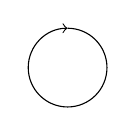
\begin{tikzpicture}
					\draw [<-] (0,0.5) arc (90:450:0.5cm);
				\end{tikzpicture}
			\end{center}
			This one rotates clockwise.
			\item \textbf{Left circularly polarized light (RCP)}. $E_{0x} = E_{0y} = E_0$ and $\delta = -\pi/2$.
			\begin{center}
				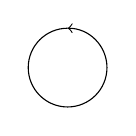
\begin{tikzpicture}
					\draw [->] (0,0.5) arc (90:450:0.5cm);
				\end{tikzpicture}
			\end{center}
			This one rotates counterclockwise.
		\end{itemize}
		These polarization states are important because
		\begin{itemize}
			\item they are relatively easy to create in a laboratory using linear and circular polarizers, and
			\item polarization measurements as well as polarization calcluations are greatly simplified using these states.
		\end{itemize}

		\item The polarization ellipse can be expressed in terms of two angular parameters: the \textbf{orientation angle} $\psi$ ($0 \leq \psi \leq \pi$) and the \textbf{ellipticity angle} $\chi$ ($-\pi/2 \leq \chi \leq \pi/4$).  The angles are given by:
		\begin{align*}
			\tan 2\psi &= \frac{2 E_{0x}E_{0y}}{E_{0x}^2 - E_{0y}^2} \cos\delta, \\
			\sin 2\chi &= \frac{2E_{0x} E_{0y}}{E_{0x}^2 + E_{0y}^2} \sin\delta.
		\end{align*}
		The above two equations can be rewritten in trigonometric terms by introducing the \textbf{auxiliary angle} $\alpha$ ($0 \leq \alpha \leq \pi/2$):
		\begin{align*}
			\tan \alpha = \frac{E_{0y}}{E_{0x}}.
		\end{align*}
		With $\alpha$, we can write $\psi$ and $\chi$ as:
		\begin{align*}
			\tan 2\psi &= (\tan 2\alpha) \cos \delta \\
			\sin 2\chi &= (\sin 2\alpha) \sin \delta.
		\end{align*}

		\item The polarization ellipse can also be represented as a point on the \textbf{Poincar\'{e} sphere}.  

		Given a polarization ellipse with parameters $\psi$ and $\chi$, the coordinate of the corresponding point on the Poincar\'{e} sphere is:
		\begin{align*}
			\begin{bmatrix}
				\cos(2\chi) \cos (2\psi) \\
				\cos(2\chi) \sin (2\psi) \\
				\sin (2\chi)
			\end{bmatrix}.
		\end{align*}
		That is, $2\chi$ is the longitudinal angle, and $2\psi$ is the azimuthal angle.  (Be careful though.  This is not the standard parameterization used in computer graphics, where the longitudinal angle runs from $0$ to $\pi$ instead of $-\pi/2$ to $\pi/2$.)

		\item Interestingly, the degenerate polarization states corresponds to important points on the Poincar\'{e} sphere:
		\begin{itemize}
			\item LHP corresponds to $(1,0,0)$.
			\item L+45P corresponds to $(0,1,0)$.
			\item LVP corresponds to $(-1,0,0)$.
			\item L-45P corresponds to $(0,-1,0)$.
			\item RCP corresponds to $(0,0,1)$.
			\item LCP corresponds to $(0,0,-1)$.
		\end{itemize}
		Moreover, all linear polarization states lie on the equator.
	\end{itemize}

	\section{The Observables of Polarized Light}

	\begin{itemize}
		\item The \textbf{Stokes polarization parameters} are 4 measurable quantitites of the polarized field.  They are defined in terms of the time average of the product of two polarization components:
		\begin{align*}
			\langle \mathcal{E}_i(z,t), \mathcal{E}_j(z,t) \rangle = \lim_{T \ra \infty} \frac{1}{T} \int_0^T \mathcal{E}_i(z,t) \mathcal{E}_j^*(z,t)\ \dee t
		\end{align*}
		where $i,j \in \{ x, y\}$, and $\,^*$ denotes complex conjugation.

		The Stokes parameters are:
		\begin{align*}
			S_0 &= \langle \mathcal{E}_x, \mathcal{E}_x  \rangle + \langle \mathcal{E}_y, \mathcal{E}_y \rangle = E_{0x}^2 + E_{0y}^2\\
			S_1 &= \langle \mathcal{E}_x, \mathcal{E}_x  \rangle - \langle \mathcal{E}_y, \mathcal{E}_y \rangle = E_{0x}^2 - E_{0y}^2 \\
			S_2 &= \langle \mathcal{E}_x, \mathcal{E}_y  \rangle + \langle \mathcal{E}_y, \mathcal{E}_x \rangle = 2 E_{0x} E_{0y} \cos\delta \\
			S_3 &= i (\langle \mathcal{E}_x, \mathcal{E}_y  \rangle - \langle \mathcal{E}_y, \mathcal{E}_x \rangle) = 2E_{0x} E_{0y} \sin\delta.
		\end{align*}

		\item It is convenient to arrange the Stokes parameters as a column matrix, which is referred to as the \textbf{Stokes vector for elliptically polarized light}:
		\begin{align*}
			S = \begin{bmatrix}
				S_0 \\
				S_1 \\
				S_2 \\
				S_3
			\end{bmatrix}
			= \begin{bmatrix}
				E_{0x}^2 + E_{0y}^2 \\
				E_{0x}^2 - E_{0y}^2 \\
				2 E_{0x} E_{0y} \cos\delta \\
				2 E_{0x} E_{0y} \sin\delta.
			\end{bmatrix}
		\end{align*}

		\item The Stokes vectors for degenerate polarization states are:
		\begin{align*}
			S_{\mathrm{LHP}} &= I_0 \begin{bmatrix}
				1 \\ 1 \\ 0 \\ 0
			\end{bmatrix} &
			S_{\mathrm{LVP}} &= I_0 \begin{bmatrix}
				1 \\ -1 \\ 0 \\ 0
			\end{bmatrix} &
			S_{\mathrm{L+45P}} &= I_0 \begin{bmatrix}
				1 \\ 0 \\ 1 \\ 0
			\end{bmatrix} \\
			S_{\mathrm{L-45P}} &= I_0 \begin{bmatrix}
				1 \\ 0 \\ -1 \\ 0
			\end{bmatrix} &
			S_{\mathrm{RCP}} &= I_0 \begin{bmatrix}
				1 \\ 0 \\ 0 \\ 1
			\end{bmatrix} &
			S_{\mathrm{LCP}} &= I_0 \begin{bmatrix}
				1 \\ 0 \\ 0 \\ -1
			\end{bmatrix}
		\end{align*}
		where $I_0$ is the intensity, which is often normalized to unity.

		Hence, they can be interpreted as follows:
		\begin{itemize}
			\item $S_0$ is the total intensity of the light beam.
			\item $S_1$ is the preponderance on LHP over LVP.
			\item $S_2$ is the preponderance on L+45P over L-45P.
			\item $S_3$ is the preponderance on RCP over LCP.
		\end{itemize}

		\item The Stokes parameters can be shown to be related to the Pointcar\'{e} sphere and the orientation and ellipticity angles as follows:
		\begin{align*}
			S_1 &= S_0 \cos(2\chi) \cos(2\psi) \\ 
			S_2 &= S_0 \cos(2\chi) \sin(2\psi) \\ 
			S_3 &= S_0 \sin(2\chi) \\
			\psi &= \frac{1}{2} \tan^{-1} \frac{S_2}{S_1} \\
			\chi &= \frac{1}{2} \sin^{-1} \frac{S_3}{S_0}.
		\end{align*}

		\item The Stokes parameters describe not only completely polarized light but also \emph{unpolarized} and \emph{partially polarized light} as well.

		\item The Stokes vector for unpolarized light is:
		\begin{align*}
			S_{\mathrm{unp}} = S_0 \begin{bmatrix}
				1 \\ 0 \\ 0 \\ 0
			\end{bmatrix}
		\end{align*}
		where $S_0$ is the first Stokes parameter (total intensity).

		\item Partially polarized light is a mizxture of completely polarized light and unpolarized light:
		\begin{align*}
			S 
			= \begin{bmatrix}
				S_0 \\ S_1 \\ S_2 \\ S_3
			\end{bmatrix}
			= (1 - \mathcal{P}) \begin{bmatrix}
				S_0 \\ 0 \\ 0 \\ 0 
			\end{bmatrix}
			+ \mathcal{P} \begin{bmatrix}
				S_0 \\ s_1 \\ s_2 \\ s_3
			\end{bmatrix}			
		\end{align*}
		where $\mathcal{P}$ ($0 \leq \mathcal{P} \leq 1$) is called the \textbf{degree of polarization} (DOP).

		\item The DOP is defined by the equation:
		\begin{align*}
			\mathcal{P} 
			= \frac{I_{\mathrm{pol}}}{I_{\mathrm{total}}}
			= \frac{\sqrt{S_1^2 + S_2^2 + S_3^3}}{S_0}
		\end{align*}

		\item Hence, for partially polarized light, we have that the following relationship holds:
		\begin{align*}
			S_0^2 \geq S_1^2+ S_2^2 + S_3^2.
		\end{align*}

		\item The Stokes parameters of a polarized beam can be measured by passing a beam sequentially through two polarizing elements know as a \textbf{wave plate} and a \textbf{polarizer}.  The emerging beam then goes to an optical detector.

		The wave plate introduces a phase shift $\phi$ between the orthogonal components of the incident beam.  The polarizer then transmits the resultant field along its transmission axis at an angle $\theta$ relative to the $x$-axis.

		The intensity $I(\theta,\phi)$ on the detect is given by:
		\begin{align*}
			I(\theta,\phi) = \frac{1}{2} (S_0 + S_1 \cos 2\theta + S_2 \sin 2\theta \cos\phi - S_3 \sin 2\theta \sin \phi).
		\end{align*}
		So, we have that
		\begin{align*}
			S_0 &= I(0,0) + I(\pi/2, 0) \\
			S_1 &= I(0,0) - I(\pi/2, 0) \\
			S_2 &= 2I(\pi/4,0) - S_0, \\
			S_3 &= S_0 - 2I(\pi/4,\pi/2).
		\end{align*}

		\item A \textbf{polarizing material} changes a light beam's polarization state as the beam propagates through it.

		Let the input beam be characterized by a Stokes vector $S$, and the output beam by $S'$.  An assumption is often made that $S$ and $S'$ are linearly related by a transformation matrix known as the \textbf{Mueller matrix}:
		\begin{align*}
			S' = MS.
		\end{align*}

		\item Polarizing elements include:
		\begin{itemize}
			\item \textbf{polarizers}, which change the amplitude,
			\item \textbf{wave plates}, which change the phase, and
			\item \textbf{rotator}, which rotates the polarizing ellipse.
		\end{itemize}
		Using thse three elements, nay elliptical polarization state can be obtained.

		\item A \textbf{linear polarizer} changes the amplitude.  It is characterized by two absorption coefficients that differ along the $x$- and $y$-axes.  The absorption coefficients in the amplitude domain are denoted by $p_x$ and $p_y$, both of which are members of $[0,1]$.

		The Mueller matrix for a linear polarizer is given by:
		\begin{align*}
			M_{\mathrm{POL}}(p_x, p_y)= \frac{1}{2} \begin{bmatrix}
				p_x^2 + p_y^2 & p_x^2 - p_y^2 & 0 & 0 \\
				p_x^2 - p_y^2 & p_x^2 + p_y^2 & 0 & 0 \\
				0 & 0 & 2p_x p_y & 0 \\
				0 & 0 & 0 & 2p_x p_y
			\end{bmatrix}
		\end{align*}

		\item For an \textbf{ideal linear polarizer}, there is complete transmission along one axis and no transmission along the other axis.

		The Mueller matrix for an ideal linear polarizer with its transmission axis along the $x$-axis is given by:
		\begin{align*}
			M_{\mathrm{POL}}(1,0) = \frac{1}{2} \begin{bmatrix}
				1 & 1 & 0 & 0 \\
				1 & 1 & 0 & 0 \\
				0 & 0 & 0 & 0 \\
				0 & 0 & 0 & 0
			\end{bmatrix}.
		\end{align*}
		On the other hand, the Mueller matrix for an ideal linear polarizer with its transmission axis along the $y$-axis is given by:
		\begin{align*}
			M_{\mathrm{POL}}(0,1) = \frac{1}{2} \begin{bmatrix}
				1 & -1 & 0 & 0 \\
				-1 & 1 & 0 & 0 \\
				0 & 0 & 0 & 0 \\
				0 & 0 & 0 & 0
			\end{bmatrix}.
		\end{align*}

		Another interesting case is the \textbf{neutral density (ND) filter}, which has the same absorption coefficients for both axes ($p_x = p_y = p$).  The Mueller matrix for the ND filter is:
		\begin{align*}
			M_{\mathrm{POL}}(p,p) = p^2 \begin{bmatrix}
				1 & 0 & 0 & 0 \\
				0 & 1 & 0 & 0 \\
				0 & 0 & 1 & 0 \\
				0 & 0 & 0 & 1
			\end{bmatrix}.
		\end{align*}
		One can see that, after the transformation, the polarization state remains the same, except for the fact that intensity is scaled down by a factor of $p^2$.

		\item Passing light through a \textbf{wave plate}, the light field experiences a phase shift of $+\phi/2$ along the $x$-axis (called the \textbf{fast axis}) and a phase shift of $-\phi/2$ along the $y$-axis (called the \textbf{slow axis}).

		The Mueller matrix for a wave plate is given by:
		\begin{align*}
			M_{\mathrm{WP}}(\phi) = \begin{bmatrix}
				1 & 0 & 0 & 0 \\
				0 & 1 & 0 & 0 \\
				0 & 0 & \cos\phi & -\sin\phi \\
				0 & 0 & \sin\phi & \cos\phi
			\end{bmatrix}.
		\end{align*}

		\item Important wave plates are the \textbf{quarter wave plate (QWP)} ($\phi = \pi/4)$ and the \textbf{half wave plate (HWP)} ($\phi = \pi/2$).  The Mueller matrices for the two wave plates are:
		\begin{align*}
			M_{QWP} &= \begin{bmatrix}
				1 & 0 & 0 & 0 \\
				0 & 1 & 0 & 0 \\
				0 & 0 & 0 & -1 \\
				0 & 0 & 1 & 0
			\end{bmatrix} \\
			M_{HWP} &= \begin{bmatrix}
				1 & 0 & 0 & 0 \\
				0 & 1 & 0 & 0 \\
				0 & 0 & -1 & 0 \\
				0 & 0 & 0 & -1
			\end{bmatrix}
		\end{align*}

		\item The QWP transforms L+45P light into RCP light and RCP light into L-45P light.

		\item The HWP changes the orientation and ellipticity angles of the incoming beam as follows:
		\begin{align*}
			\begin{bmatrix}
				1 & 0 & 0 & 0 \\
				0 & 1 & 0 & 0 \\
				0 & 0 & -1 & 0 \\
				0 & 0 & 0 & -1
			\end{bmatrix}
			\begin{bmatrix}
				1 \\
				\cos 2\chi \cos 2\psi \\
				\cos 2\chi \sin 2\psi \\
				\sin 2\chi
			\end{bmatrix}
			= \begin{bmatrix}
				1 \\
				\cos 2\chi \cos 2\psi \\
				-\cos 2\chi \sin 2\psi \\
				-\sin 2\chi
			\end{bmatrix}
			= \begin{bmatrix}
				1 \\
				\cos 2(\chi - \pi/2) \cos 2(\pi/2 - \psi) \\
				\cos 2(\chi - \pi/2) \sin 2(\pi/2 - \psi) \\
				\sin 2(\chi - \pi/2).
			\end{bmatrix}
		\end{align*}

		\item The Mueller matrix of a \textbf{rotator} is given by:
		\begin{align*}
			M_{\mathrm{ROM}}(\theta) = \begin{bmatrix}
				1 & 0 & 0 & 0 \\
				0 & \cos 2\theta & \sin 2\theta & 0 \\
				0 & -\sin 2\theta & \cos 2\theta & 0 \\
				0 & 0 & 0 & 1
			\end{bmatrix}
		\end{align*}
		where $\theta$ is the angle of rotation.  A rotator only rotates the polarization ellipse.  It does not affect the ellipticity:
		\begin{align*}
			\begin{bmatrix}
				1 & 0 & 0 & 0 \\
				0 & \cos 2\theta & \sin 2\theta & 0 \\
				0 & -\sin 2\theta & \cos 2\theta & 0 \\
				0 & 0 & 0 & 1
			\end{bmatrix}
			\begin{bmatrix}
				1 \\
				\cos 2\chi \cos 2\psi \\
				\cos 2\chi \sin 2\psi \\
				\sin 2\chi
			\end{bmatrix}
			= \begin{bmatrix}
				1 \\
				\cos 2\chi \cos (2\psi + 2\theta) \\
				\cos 2\chi \sin (2\psi + 2\theta) \\
				\sin 2\chi
			\end{bmatrix}
		\end{align*}

		\item All matrices discussed so far are defined with the canonical coordiante system with the standard $x$- and $y$-axis.  That is, it is assumed that the polarizing element is aligned with the canonical coordinate system.  If the element is rotated by an angle of $\theta$ wrt the canonical coordinate system, then the Mueller matrix of the rotated polarizing element is given by:
		\begin{align*}
			M(\theta) = M_{\mathrm{ROT}}(-\theta)\, M \, M_{\mathrm{ROT}}(\theta).
		\end{align*}

		\item The Mueller matrix for a rotated ideal linear polarizer is
		\begin{align*}
			M_{\mathrm{POL}}(\theta) = \frac{1}{2} \begin{bmatrix}
				1 & \cos 2\theta & \sin 2\theta & 0 \\
				\cos 2\theta & \cos^2 2\theta & \sin 2\theta \cos 2\theta & 0 \\
				\sin 2\theta & \sin 2\theta \cos 2\theta & \sin^2 2\theta & 0 \\
				0 & 0 & 0 & 0
			\end{bmatrix}.
		\end{align*}
		The Stokes vector of the output beam is given by:
		\begin{align*}
			\frac{1}{2} \begin{bmatrix}
				1 & \cos 2\theta & \sin 2\theta & 0 \\
				\cos 2\theta & \cos^2 2\theta & \sin 2\theta \cos 2\theta & 0 \\
				\sin 2\theta & \sin 2\theta \cos 2\theta & \sin^2 2\theta & 0 \\
				0 & 0 & 0 & 0
			\end{bmatrix}
			\begin{bmatrix}
				S_0 \\ S_1 \\ S_2 \\ S_3
			\end{bmatrix}
			= \frac{1}{2}(S_0 + S_1 \cos 2\theta + S_2 \sin 2\theta) \begin{bmatrix}
				1 \\ \cos 2\theta \\ \sin 2\theta \\ 0
			\end{bmatrix}.			
		\end{align*}
		So, regardless of the polarization state of the input beam, the output beam does not have circular polarization component.

		\item For $\theta = 0^\circ$, $45^\circ$, $90^\circ$, and $135^\circ$, the Mueller matrix reduces to the following special forms:
		\begin{align*}
			M_{\mathrm{LHP}} &= M_{\mathrm{POL}}(0^\circ) = \frac{1}{2} \begin{bmatrix}
				1 & 1 & 0 & 0 \\
				1 & 1 & 0 & 0 \\
				0 & 0 & 0 & 0 \\
				0 & 0 & 0 & 0
			\end{bmatrix} &
			M_{\mathrm{L+45P}} &= M_{\mathrm{POL}}(45^\circ) = \frac{1}{2} \begin{bmatrix}
				1 & 0 & 1 & 0 \\
				0 & 0 & 0 & 0 \\
				1 & 0 & 1 & 0 \\
				0 & 0 & 0 & 0
			\end{bmatrix} \\
			M_{\mathrm{LVP}} &= M_{\mathrm{POL}}(90^\circ) = \frac{1}{2} \begin{bmatrix}
				1 & -1 & 0 & 0 \\
				-1 & 1 & 0 & 0 \\
				0 & 0 & 0 & 0 \\
				0 & 0 & 0 & 0
			\end{bmatrix} &
			M_{\mathrm{L-45P}} &= M_{\mathrm{POL}}(135^\circ) = \frac{1}{2} \begin{bmatrix}
				1 & 0 & -1 & 0 \\
				0 & 0 & 0 & 0 \\
				-1 & 0 & 1 & 0 \\
				0 & 0 & 0 & 0
			\end{bmatrix}
		\end{align*}

		\item A circular plarizer is constructed from an L+45P polarizer and a QWP.  The Mueller matrix of a circular polarizer is given by:
		\begin{align*}
			M_{\mathrm{CP}} 
			= M_{\mathrm{QWP}} M_{\mathrm{L+45P}}
			= \begin{bmatrix}
				1 & 0 & 1 & 0 \\
				0 & 0 & 0 & 0 \\
				0 & 0 & 0 & 0 \\
				1 & 0 & 1 & 0 
			\end{bmatrix}.
		\end{align*}
		We have that
		\begin{align*}
			\begin{bmatrix}
				1 & 0 & 1 & 0 \\
				0 & 0 & 0 & 0 \\
				0 & 0 & 0 & 0 \\
				1 & 0 & 1 & 0 
			\end{bmatrix}
			\begin{bmatrix}
				S_0 \\
				S_1 \\
				S_2 \\
				S_3
			\end{bmatrix}
			= \frac{1}{2} (S_0 + S_2) \begin{bmatrix}
				1 \\ 0 \\ 0 \\ 1
			\end{bmatrix}.
		\end{align*}
		So, the output beam is always circularly polarized regardless of the polarization state of the input beam.
	\end{itemize}

	\section{Reflection and Transmission}

	\begin{itemize}
		\item Consider the plane in which light reflects off and refracts into a dielectric material.  Let us set the coordinate system so that the two components are the one that is parallel to the plane (p-polarization) and the one that is perpendicular to the plane (s-polarization).

		\item Let $i$ and $r$ be the incident angle and the refraction angle, respectively.  The amplitudes of the reflected and refracted rays are governed by \textbf{Fresnel's equations}:
		\begin{align*}
			R_p &= \frac{\tan (i-r)}{\tan (i+r)} E_p, &
			R_s &= \frac{\sin (i-r)}{\sin (i+r)} E_s \\
			T_p &= \frac{2\sin r \cos i}{\sin(i+r)\cos(i-r)} E_p, &
			T_s &= \frac{2\sin r \cos i}{\sin (i+r)} E_s.
		\end{align*}

		\item The Stokes parameters for the reflected light in terms of the Stokes parameters of the incoming light are given by:
		\begin{align*}
			S_{0R} &= f_R [(\cos^2 (i-r) + \cos^2 (i+r))S_0 + (\cos^2 (i-r) - \cos^2 (i+r)) S_1] \\
			S_{1R} &= f_R [(\cos^2 (i-r) - \cos^2 (i+r))S_0 + (\cos^2 (i-r) + \cos^2 (i+r)) S_1] \\
			S_{2R} &= -f_R(2\cos(i-r) \cos(i+r)) S_2 \\
			S_{3R} &= -f_R(2\cos(i-r) \cos(i+r)) S_3
		\end{align*}
		where
		\begin{align*}
			f_R = \frac{1}{2} \bigg( \frac{\tan (i-r)}{\sin (i+r)} \bigg)^2.
		\end{align*}
		So, the Mueller matrix for reflection is:
		\begin{align*}
			M_R &= f_R \begin{bmatrix}
				\cos^2 (i-r) + \cos^2 (i+1) & \cos^2 (i-r) - \cos^2 (i+1) & 0 & 0 \\
				\cos^2 (i-r) - \cos^2 (i+1) & \cos^2 (i-r) + \cos^2 (i+1) & 0 & 0 \\
				0 & 0 & -2 \cos(i-r) \cos(i+r) & 0 \\
				0 & 0 & 0 & -2\cos(i-r)\cos(i+r) 
			\end{bmatrix}
		\end{align*}

		\item The Stokes parameters for the refracted light in terms of the Stokes parameters of the incoming light are given by:
		\begin{align*}
			S_{0T} &= f_T[(\cos^2(i-r) + 1)S_0 + (\cos^2 (i-r) - 1) S_1]\\
			S_{1T} &= f_T[(\cos^2(i-r) - 1)S_0 + (\cos^2 (i-r) + 1) S_1] \\
			S_{2T} &= -f_T(2\cos(i-r)) S_2 \\
			S_{3T} &= -f_T(2\cos(i-r)) S_3 
		\end{align*}
		where
		\begin{align*}
			f_T = \frac{1}{2} \frac{\sin 2i \sin 2r}{(\sin(i+r)\cos(i-r))^2}.
		\end{align*}
		So, the Mueller matrix for refraction is:
		\begin{align*}
			M_T = f_T \begin{bmatrix}
				\cos^2(i-r)+1 & \cos^2(i-r)-1 & 0 & \\
				\cos^2(i-r)-1 & \cos^2(i-r)+1 & 0 & \\
				0 & 0 & -2\cos(i-r) & 0 \\
				0 & 0 & 0 & -2\cos(i-r)
			\end{bmatrix}.
		\end{align*}

		\item We have that $S_0 = S_{0R} + S_{0T}$, which means that the total energy is conserved (as it should be).

		\item Consider the behavior of unpolarized light after it reflects from the surface.
		\begin{align*}
			S_R = M_R \begin{bmatrix}
				1 \\ 0 \\ 0 \\ 0
			\end{bmatrix}
			= \frac{1}{2} \bigg( \frac{\tan (i-r)}{\tan (i+r)} \bigg)^2 \begin{bmatrix}
				\cos^2 (i-r) + \cos^2 (i+r) \\
				\cos^2 (i-r) - \cos^2 (i+r) \\
				0 \\
				0 
			\end{bmatrix}.
		\end{align*}
		The degree of polarization $\mathcal{P}$ is given by:
		\begin{align*}
			\mathcal{P} 
			= \bigg| \frac{S_{1R}}{S_{0R}} \bigg| 
			= \bigg| \frac{\cos^2 (i-r) - \cos^2(i+r)}{\cos^2(i-r) + \cos^2 (i+r)} \bigg|.
		\end{align*}
		In general, $\mathcal{P}$ is less than $1$.  If, however, $\cos (i+r) = 0$, then $\mathcal{P} = 1$ and $i+r = \pi/2$.  This is the Brewster's angle, and $S_R$ is reduced to:
		\begin{align*}
			S_R = \frac{1}{2} \cos^2 2i \begin{bmatrix}
				1 \\ 1 \\ 0 \\ 0
			\end{bmatrix}.
		\end{align*}
		That is, at Brewster's angle, the reflected light is LHP and the LVP component vanishes.  So, if the beam passes through an LVP filter, the intensity of the beam that emerges is $0$.

		\item Now, consider the behavior of unpolarized light after it transmits into the material.  We have that:
		\begin{align*}
			S_T 
			= M_T \begin{bmatrix}
				1 \\ 0 \\ 0 \\ 0
			\end{bmatrix}
			= \frac{1}{2} \frac{\sin 2i \sin 2r}{2(\sin(i+r) \cos(i-r))^2}
			\begin{bmatrix}
				\cos^2 2(i-r) + 1 \\
				\cos^2 2(i-r) - 1 \\
				0 \\
				0
			\end{bmatrix}
		\end{align*}
		The DOP of the transmitted light is:
		\begin{align*}
			\mathcal{P} 
			= \bigg| \frac{S_{1T}}{S_{0T}} \bigg| 
			= \bigg| \frac{\cos^2(i-r)-1}{\cos^2(i-r) + 1} \bigg|.
		\end{align*}
		The transmitted light is always partially polarized.

		\item When light propagates from a material with higher index of refraction (say $n$) to one with lower index of refraction (say $1$),  total internal reflection occurs when $n \sin i > 1$.  The reflected light experiences the following phase shift.  The Mueller matrix is given by:
		\begin{align*}
			M_R = \begin{bmatrix}
				1 & 0 & 0 & 0 \\
				0 & 1 & 0 & 0 \\
				0 & 0 & \cos\delta & -\sin\delta \\
				0 & 0 & \sin\delta & \cos\delta
			\end{bmatrix}			
		\end{align*}
		where
		\begin{align*}
			\tan \frac{\delta}{2} = \frac{\cos i \sqrt{n^2 \sin^2 i - 1}}{n \sin^2 i}.
		\end{align*}

		\item A simpler notation for the Mueller matrices for reflection and transmission uses the \textbf{Fresnel reflection and transmission coefficients}.  

		The Fresnel reflection coefficients are:
		\begin{align*}
			\rho_s &= \bigg( \frac{R_s}{E_s} \bigg)^2 = \bigg( \frac{\sin (i-r)}{\sin (i+r)} \bigg)^2, \\
			\rho_p & = \bigg( \frac{R_p}{E_p} \bigg)^2 = \bigg( \frac{\tan (i-r)}{\tan (i+r)} \bigg)^2.
		\end{align*}

		The Fresnel transmission coefficients are:
		\begin{align*}
			\tau_s &= \frac{n \cos r}{\cos i} \bigg( \frac{T_s}{E_s} \bigg)^2 = \frac{\sin 2i \sin 2r}{\sin^2(i+r)} \\			
			\tau_p &= \frac{n \cos r}{\cos i} \bigg( \frac{T_p}{E_p} \bigg)^2 = \frac{\sin 2i \sin 2r}{\sin^2 (i+r) \cos^2 (i-r)}.
		\end{align*}

		Note that $\rho_s + \tau_s = 1$ and $\rho_p + \tau_p = 1$.

		\item At the Brewster angle $i_B$, the Fresnel coefficients are:
		\begin{align*}
			\rho_{s,B} &= \cos^2 2i_B, &
			\rho_{p,B} &= 0, &
			\tau_{s,B} &= \sin^2 2i_B, &
			\tau_{p,B} &= 1 
		\end{align*}

		\item The Mueller matrices for reflection and transmission are given by:
		\begin{align*}
			M_r &= \frac{1}{2} \begin{bmatrix}
				\rho_s + \rho_p & \rho_s - \rho_p & 0 & 0 \\
				\rho_s - \rho_p & \rho_s + \rho_p & 0 & 0 \\
				0 & 0 & 2\sqrt{\rho_s \rho_p} & 0 \\
				0 & 0 & 0 & 2\sqrt{\rho_s \rho_p}
			\end{bmatrix} \\
			M_t &= \frac{1}{2} \begin{bmatrix}
				\tau_s + \tau_p & \tau_s - \tau_p & 0 & 0 \\
				\tau_s - \tau_p & \tau_s + \tau_p & 0 & 0 \\
				0 & 0 & 2\sqrt{\tau_s \tau_p} & 0 \\
				0 & 0 & 0 & 2\sqrt{\tau_s \tau_p}
			\end{bmatrix}
		\end{align*}
	\end{itemize}

	\section{Other Polarization Matrix Calculi}

	\subsection{The Jones Matrix Calculus}

	\begin{itemize}
		\item  The \textbf{Jones matrix calculus} is a matrix formulation of polarized light that consists of $2\times 1$ \textbf{Jones vectors} to describe the field components and $2 \times 2$ \textbf{Jones matrices} to describe polarizing components.

		\item It is simpler than the Mueller calculus and is limited to treating only completely polarized light.  It is used when treating interference phenomena or in problems where field amplitudes must be superposed.

		\item The $2 \times 1$ Jones vector for polarized light field is:
		\begin{align*}
			\ve{E} = \begin{bmatrix}
				\mathcal{E}_x \\ \mathcal{E}_y
			\end{bmatrix}
			= \begin{bmatrix}
				E_{0x} e^{i\delta_x} \\
				E_{0y} e^{i\delta_y}
			\end{bmatrix}
		\end{align*}
		where $E_{0x}$ and $E_{0y}$ are the amplitudes, and $\delta_x$ and $\delta_y$ are the phases.

		\item Intensity $I$ of the field can be calculated by dotting the Jones vector:
		\begin{align*}
			I = \begin{bmatrix}
				\mathcal{E}_x^* & \mathcal{E}_y^*
			\end{bmatrix}
			\begin{bmatrix}
				\mathcal{E}_x \\
				\mathcal{E}_y
			\end{bmatrix}
			= \mathcal{E}_x^* \mathcal{E}_x + \mathcal{E}^*_y \mathcal{E}_y
			= \mathbf{E}^H \mathbf{E}.
		\end{align*}

		\item The Jones vectors for the degenerate polarization states are:
		\begin{align*}
			\mathbf{E}_{\mathrm{LHP}} &= \begin{bmatrix}
				1 \\ 0
			\end{bmatrix} &
			\mathbf{E}_{\mathrm{LVP}} &= \begin{bmatrix}
				0 \\ 1
			\end{bmatrix} \\
			\mathbf{E}_{\mathrm{L+45P}} &= \frac{1}{\sqrt{2}} \begin{bmatrix}
				1 \\ 1
			\end{bmatrix} &
			\mathbf{E}_{\mathrm{L-45P}} &= \frac{1}{\sqrt{2}} \begin{bmatrix}
				1 \\ -1
			\end{bmatrix} \\
			\mathbf{E}_{\mathrm{RCP}} &= \frac{1}{\sqrt{2}} \begin{bmatrix}
				1 \\ i
			\end{bmatrix} &
			\mathbf{E}_{\mathrm{LCP}} &= \frac{1}{\sqrt{2}} \begin{bmatrix}
				1 \\ -i
			\end{bmatrix}
		\end{align*}

		\item Given an arbitrary polarized light, we can decompose it into $\mathbf{E}_{\mathrm{LHP}}$ and $\mathbf{E}_{\mathrm{LVP}}$:
		\begin{align*}
			\mathbf{E} 
			&= \begin{bmatrix}
				E_{0x} e^{i\delta_x} \\
				E_{0y} e^{i\delta_y}
			\end{bmatrix}
			= E_{0x} e^{i\delta_x} \begin{bmatrix} 1 \\ 0 \end{bmatrix}
			+ E_{0y} e^{i\delta_y} \begin{bmatrix} 0 \\ 1 \end{bmatrix}
			= E_{0x} e^{i\delta_x} \ve{E}_{\mathrm{LHP}}
			+ E_{0y} e^{i\delta_y} \ve{E}_{\mathrm{LVP}}.
		\end{align*}		

		\item A polarizing element is represented by a $2\times 2$ Jones matrix:
		\begin{align*}
			J = \begin{bmatrix}
				j_{xx} & j_{xy} \\
				j_{yx} & j_{yy}
			\end{bmatrix}
		\end{align*}

		\item For a linear polarizer, the Jones matrix is:
		\begin{align*}
			J_{\mathrm{POL}} &= \begin{bmatrix}
				p_x & 0 \\
				0 & p_y
			\end{bmatrix}			
		\end{align*}
		where $0 \leq p_x, p_y \leq 1$.

		For an ideal linear horizontal and linear vertical polarizer, the Jones matrices tkae the form, respectively:
		\begin{align*}
			J_{\mathrm{LHP}} &= \begin{bmatrix}
				1 & 0 \\ 0 & 0
			\end{bmatrix} &
			J_{\mathrm{LVP}} &= \begin{bmatrix}
				0 & 0 \\ 0 & 1
			\end{bmatrix}.
		\end{align*}

		\item The Jones matrices for a wave plate with a phase shift of $\phi/2$ along the $x$-axis and $-\phi/2$ along the $y$-axis is:
		\begin{align*}
			J_{\mathrm{WP}} &= \begin{bmatrix}
				e^{i \phi/2} & 0 \\
				0 & e^{-i\phi/2}
			\end{bmatrix},
		\end{align*}
		and the above is equivalent (modulo the absolute phase) to:
		\begin{align*}
			\begin{bmatrix}
				1 & 0 \\
				0 & e^{-i\phi}
			\end{bmatrix}
		\end{align*}

		The Jones matrices for QWP and HWP are:
		\begin{align*}
			J_{QWP} &= \begin{bmatrix}
				1 & 0 \\
				0 & -i
			\end{bmatrix} &
			J_{HWP} &= \begin{bmatrix}
				1 & 0 \\
				0 & -1
			\end{bmatrix}.
		\end{align*}

		\item The Jones matrix for a rotator is:
		\begin{align*}
			J_{\mathrm{ROT}}(\theta) = \begin{bmatrix}
				\cos \theta & \sin \theta \\
				-\sin \theta & \cos \theta
			\end{bmatrix}.
		\end{align*}
	\end{itemize}

	\subsection{Wolf's Coherency Matrix Calculus}

	\begin{itemize}
		\item The \textbf{Wolf's coherency matrix calculus} serves as a usefu bridge between the Mueller and Jones matrix calculi.

		\item The coherency matrix C is deinfed in terms of the complex product of the optical field:
		\begin{align*}
			C &= \begin{bmatrix}
				C_{xx} & C_{xy} \\
				C_{yx} & C_{yy}
			\end{bmatrix}
			= \begin{bmatrix}
				\langle \mathcal{E}_x, \mathcal{E}_x \rangle & \langle \mathcal{E}_x, \mathcal{E}_y \rangle \\
				\langle \mathcal{E}_y, \mathcal{E}_x \rangle & \langle \mathcal{E}_y, \mathcal{E}_y \rangle
			\end{bmatrix} \\			
			&= \frac{1}{2} \begin{bmatrix}
				S_0 + S_1 & S_2 + iS_3 \\
				S_2 - iS_3 & S_0 - S_1
			\end{bmatrix} 
		 	= \frac{1}{2} \bigg( 
		 		S_1 \begin{bmatrix}
		 			1 & 0 \\ 0 & 1
		 		\end{bmatrix}
		 		+ S_2 \begin{bmatrix}
		 			1 & 0 \\ 0 & -1
		 		\end{bmatrix}
		 		+ S_3 \begin{bmatrix}
		 			0 & 1 \\ 1 & 0
		 		\end{bmatrix}
		 		+ S_4 \begin{bmatrix}
		 			0 & i \\ -i & 0
		 		\end{bmatrix}
		 	\bigg).
		\end{align*}
		Here, the 4 basis matrices are called the \textbf{Pauli spin matrices}.

		\item The matrices of degenerate polarization states are:
		\begin{align*}
			C_{\mathrm{LHP}} &= \frac{1}{2} \begin{bmatrix}
				1 & 0 \\ 0 & 0
			\end{bmatrix} &
			C_{\mathrm{LVP}} &= \frac{1}{2} \begin{bmatrix}
				0 & 0 \\ 0 & 1
			\end{bmatrix} \\
			C_{\mathrm{L+45P}} &= \frac{1}{2} \begin{bmatrix}
				1 & 1 \\ 1 & 1
			\end{bmatrix} &
			C_{\mathrm{L-45P}} &= \frac{1}{2} \begin{bmatrix}
				1 & -1 \\ -1 & 1
			\end{bmatrix} \\
			C_{\mathrm{RCP}} &= \frac{1}{2} \begin{bmatrix}
				1 & i \\ -i & 1
			\end{bmatrix} &
			C_{\mathrm{LCP}} &= \frac{1}{2} \begin{bmatrix}
				1 & -i \\ i & 1
			\end{bmatrix}.
		\end{align*}

		\item The matrix for unpolarized light is given by:
		\begin{align*}
			C_{\mathrm{UNP}} = \frac{1}{2} \begin{bmatrix}
				1 & 0 \\ 0 & 1
			\end{bmatrix},
		\end{align*}
		and the general matrix for elliptically polarized light is given by:
		\begin{align*}
			C_{\mathrm{ELP}} = \frac{1}{2} \begin{bmatrix}
				1 + \cos 2\alpha & e^{i\delta} \sin 2\alpha \\
				e^{-i\delta} \sin 2\alpha & 1 - \cos 2\alpha
			\end{bmatrix}
		\end{align*}
		where $\alpha = \tan^{-1} (E_{0y}/E_{0x})$ and $\delta$ is the phase.
	\end{itemize}	

	\bibliographystyle{apalike}
	\bibliography{polarization}  
\end{document}